\documentclass[12pt,a4paper]{article}

\usepackage[a4paper,text={16.5cm,25.2cm},centering]{geometry}
\usepackage{lmodern}
\usepackage{amssymb,amsmath}
\usepackage{bm}
\usepackage{graphicx}
\usepackage{microtype}
\usepackage{hyperref}
\setlength{\parindent}{0pt}
\setlength{\parskip}{1.2ex}

\hypersetup
       {   pdfauthor = {  },
           pdftitle={  },
           colorlinks=TRUE,
           linkcolor=black,
           citecolor=blue,
           urlcolor=blue
       }




\usepackage{upquote}
\usepackage{listings}
\usepackage{xcolor}
\lstset{
    basicstyle=\ttfamily\footnotesize,
    upquote=true,
    breaklines=true,
    breakindent=0pt,
    keepspaces=true,
    showspaces=false,
    columns=fullflexible,
    showtabs=false,
    showstringspaces=false,
    escapeinside={(*@}{@*)},
    extendedchars=true,
}
\newcommand{\HLJLt}[1]{#1}
\newcommand{\HLJLw}[1]{#1}
\newcommand{\HLJLe}[1]{#1}
\newcommand{\HLJLeB}[1]{#1}
\newcommand{\HLJLo}[1]{#1}
\newcommand{\HLJLk}[1]{\textcolor[RGB]{148,91,176}{\textbf{#1}}}
\newcommand{\HLJLkc}[1]{\textcolor[RGB]{59,151,46}{\textit{#1}}}
\newcommand{\HLJLkd}[1]{\textcolor[RGB]{214,102,97}{\textit{#1}}}
\newcommand{\HLJLkn}[1]{\textcolor[RGB]{148,91,176}{\textbf{#1}}}
\newcommand{\HLJLkp}[1]{\textcolor[RGB]{148,91,176}{\textbf{#1}}}
\newcommand{\HLJLkr}[1]{\textcolor[RGB]{148,91,176}{\textbf{#1}}}
\newcommand{\HLJLkt}[1]{\textcolor[RGB]{148,91,176}{\textbf{#1}}}
\newcommand{\HLJLn}[1]{#1}
\newcommand{\HLJLna}[1]{#1}
\newcommand{\HLJLnb}[1]{#1}
\newcommand{\HLJLnbp}[1]{#1}
\newcommand{\HLJLnc}[1]{#1}
\newcommand{\HLJLncB}[1]{#1}
\newcommand{\HLJLnd}[1]{\textcolor[RGB]{214,102,97}{#1}}
\newcommand{\HLJLne}[1]{#1}
\newcommand{\HLJLneB}[1]{#1}
\newcommand{\HLJLnf}[1]{\textcolor[RGB]{66,102,213}{#1}}
\newcommand{\HLJLnfm}[1]{\textcolor[RGB]{66,102,213}{#1}}
\newcommand{\HLJLnp}[1]{#1}
\newcommand{\HLJLnl}[1]{#1}
\newcommand{\HLJLnn}[1]{#1}
\newcommand{\HLJLno}[1]{#1}
\newcommand{\HLJLnt}[1]{#1}
\newcommand{\HLJLnv}[1]{#1}
\newcommand{\HLJLnvc}[1]{#1}
\newcommand{\HLJLnvg}[1]{#1}
\newcommand{\HLJLnvi}[1]{#1}
\newcommand{\HLJLnvm}[1]{#1}
\newcommand{\HLJLl}[1]{#1}
\newcommand{\HLJLld}[1]{\textcolor[RGB]{148,91,176}{\textit{#1}}}
\newcommand{\HLJLs}[1]{\textcolor[RGB]{201,61,57}{#1}}
\newcommand{\HLJLsa}[1]{\textcolor[RGB]{201,61,57}{#1}}
\newcommand{\HLJLsb}[1]{\textcolor[RGB]{201,61,57}{#1}}
\newcommand{\HLJLsc}[1]{\textcolor[RGB]{201,61,57}{#1}}
\newcommand{\HLJLsd}[1]{\textcolor[RGB]{201,61,57}{#1}}
\newcommand{\HLJLsdB}[1]{\textcolor[RGB]{201,61,57}{#1}}
\newcommand{\HLJLsdC}[1]{\textcolor[RGB]{201,61,57}{#1}}
\newcommand{\HLJLse}[1]{\textcolor[RGB]{59,151,46}{#1}}
\newcommand{\HLJLsh}[1]{\textcolor[RGB]{201,61,57}{#1}}
\newcommand{\HLJLsi}[1]{#1}
\newcommand{\HLJLso}[1]{\textcolor[RGB]{201,61,57}{#1}}
\newcommand{\HLJLsr}[1]{\textcolor[RGB]{201,61,57}{#1}}
\newcommand{\HLJLss}[1]{\textcolor[RGB]{201,61,57}{#1}}
\newcommand{\HLJLssB}[1]{\textcolor[RGB]{201,61,57}{#1}}
\newcommand{\HLJLnB}[1]{\textcolor[RGB]{59,151,46}{#1}}
\newcommand{\HLJLnbB}[1]{\textcolor[RGB]{59,151,46}{#1}}
\newcommand{\HLJLnfB}[1]{\textcolor[RGB]{59,151,46}{#1}}
\newcommand{\HLJLnh}[1]{\textcolor[RGB]{59,151,46}{#1}}
\newcommand{\HLJLni}[1]{\textcolor[RGB]{59,151,46}{#1}}
\newcommand{\HLJLnil}[1]{\textcolor[RGB]{59,151,46}{#1}}
\newcommand{\HLJLnoB}[1]{\textcolor[RGB]{59,151,46}{#1}}
\newcommand{\HLJLoB}[1]{\textcolor[RGB]{102,102,102}{\textbf{#1}}}
\newcommand{\HLJLow}[1]{\textcolor[RGB]{102,102,102}{\textbf{#1}}}
\newcommand{\HLJLp}[1]{#1}
\newcommand{\HLJLc}[1]{\textcolor[RGB]{153,153,119}{\textit{#1}}}
\newcommand{\HLJLch}[1]{\textcolor[RGB]{153,153,119}{\textit{#1}}}
\newcommand{\HLJLcm}[1]{\textcolor[RGB]{153,153,119}{\textit{#1}}}
\newcommand{\HLJLcp}[1]{\textcolor[RGB]{153,153,119}{\textit{#1}}}
\newcommand{\HLJLcpB}[1]{\textcolor[RGB]{153,153,119}{\textit{#1}}}
\newcommand{\HLJLcs}[1]{\textcolor[RGB]{153,153,119}{\textit{#1}}}
\newcommand{\HLJLcsB}[1]{\textcolor[RGB]{153,153,119}{\textit{#1}}}
\newcommand{\HLJLg}[1]{#1}
\newcommand{\HLJLgd}[1]{#1}
\newcommand{\HLJLge}[1]{#1}
\newcommand{\HLJLgeB}[1]{#1}
\newcommand{\HLJLgh}[1]{#1}
\newcommand{\HLJLgi}[1]{#1}
\newcommand{\HLJLgo}[1]{#1}
\newcommand{\HLJLgp}[1]{#1}
\newcommand{\HLJLgs}[1]{#1}
\newcommand{\HLJLgsB}[1]{#1}
\newcommand{\HLJLgt}[1]{#1}


\begin{document}



\begin{lstlisting}
(*@\HLJLnf{include}@*)(*@\HLJLp{(}@*)(*@\HLJLs{"{}../../../code/sfd.jl"{}}@*)(*@\HLJLp{)}@*)
(*@\HLJLk{using}@*) (*@\HLJLoB{.}@*)(*@\HLJLn{SpaceFlightDynamics}@*)
(*@\HLJLk{using}@*) (*@\HLJLn{Plots}@*)
(*@\HLJLnf{plotlyjs}@*)(*@\HLJLp{()}@*)

(*@\HLJLcs{{\#}}@*) (*@\HLJLcs{Case}@*) (*@\HLJLcs{1:}@*) (*@\HLJLcs{short‐way}@*)
(*@\HLJLn{r1{\_}c1}@*) (*@\HLJLoB{=}@*) (*@\HLJLp{[}@*)(*@\HLJLnfB{8000.0}@*)(*@\HLJLp{,}@*) (*@\HLJLnfB{0.0}@*)(*@\HLJLp{,}@*) (*@\HLJLnfB{0.0}@*)(*@\HLJLp{]}@*)
(*@\HLJLn{r2{\_}c1}@*) (*@\HLJLoB{=}@*) (*@\HLJLp{[}@*)(*@\HLJLnfB{7000.0}@*)(*@\HLJLp{,}@*) (*@\HLJLnfB{7000.0}@*)(*@\HLJLp{,}@*) (*@\HLJLnfB{0.0}@*)(*@\HLJLp{]}@*)
(*@\HLJLn{TOF{\_}c1}@*) (*@\HLJLoB{=}@*) (*@\HLJLnfB{3600.0}@*)

(*@\HLJLn{v1{\_}c1}@*)(*@\HLJLp{,}@*) (*@\HLJLn{v2{\_}c1}@*)(*@\HLJLp{,}@*) (*@\HLJLn{e{\_}c1}@*)(*@\HLJLp{,}@*) (*@\HLJLn{rp{\_}c1}@*) (*@\HLJLoB{=}@*) (*@\HLJLnf{solve{\_}lambert}@*)(*@\HLJLp{(}@*)(*@\HLJLn{r1{\_}c1}@*)(*@\HLJLp{,}@*) (*@\HLJLn{r2{\_}c1}@*)(*@\HLJLp{,}@*) (*@\HLJLn{TOF{\_}c1}@*)(*@\HLJLp{;}@*) (*@\HLJLn{long{\_}way}@*)(*@\HLJLoB{=}@*)(*@\HLJLkc{false}@*)(*@\HLJLp{)}@*)
(*@\HLJLn{sv{\_}c1}@*) (*@\HLJLoB{=}@*) (*@\HLJLnf{solve{\_}2BP}@*)(*@\HLJLp{(}@*)(*@\HLJLnf{StateVectors}@*)(*@\HLJLp{(}@*)(*@\HLJLn{r1{\_}c1}@*)(*@\HLJLp{,}@*) (*@\HLJLn{v1{\_}c1}@*)(*@\HLJLp{),}@*) (*@\HLJLp{(}@*)(*@\HLJLnfB{0.0}@*)(*@\HLJLp{,}@*) (*@\HLJLn{TOF{\_}c1}@*)(*@\HLJLp{),}@*) (*@\HLJLn{\ensuremath{\mu}}@*)(*@\HLJLoB{=}@*)(*@\HLJLn{\ensuremath{\mu}{\_}Earth}@*)(*@\HLJLp{,}@*) (*@\HLJLn{int{\_}pts}@*) (*@\HLJLoB{=}@*) (*@\HLJLni{500}@*)(*@\HLJLp{)}@*)

(*@\HLJLn{r2{\_}c1{\_}diff}@*) (*@\HLJLoB{=}@*) (*@\HLJLn{r2{\_}c1}@*) (*@\HLJLoB{-}@*) (*@\HLJLn{sv{\_}c1}@*)(*@\HLJLp{[}@*)(*@\HLJLk{end}@*)(*@\HLJLp{]}@*)(*@\HLJLoB{.}@*)(*@\HLJLn{r}@*)
(*@\HLJLn{v2{\_}c1{\_}diff}@*) (*@\HLJLoB{=}@*) (*@\HLJLn{v2{\_}c1}@*) (*@\HLJLoB{-}@*) (*@\HLJLn{sv{\_}c1}@*)(*@\HLJLp{[}@*)(*@\HLJLk{end}@*)(*@\HLJLp{]}@*)(*@\HLJLoB{.}@*)(*@\HLJLn{v}@*)

(*@\HLJLnf{println}@*)(*@\HLJLp{(}@*)(*@\HLJLs{"{}Case}@*) (*@\HLJLs{1}@*) (*@\HLJLs{Final}@*) (*@\HLJLs{Position}@*) (*@\HLJLs{Vector}@*) (*@\HLJLs{Diff:}@*) (*@\HLJLs{"{}}@*)(*@\HLJLp{,}@*) (*@\HLJLn{r2{\_}c1{\_}diff}@*)(*@\HLJLp{)}@*)
(*@\HLJLnf{println}@*)(*@\HLJLp{(}@*)(*@\HLJLs{"{}Case}@*) (*@\HLJLs{1}@*) (*@\HLJLs{Final}@*) (*@\HLJLs{Velocity}@*) (*@\HLJLs{Vector}@*) (*@\HLJLs{Diff:}@*) (*@\HLJLs{"{}}@*)(*@\HLJLp{,}@*) (*@\HLJLn{v2{\_}c1{\_}diff}@*)(*@\HLJLp{)}@*)

(*@\HLJLcs{{\#}}@*) (*@\HLJLcs{Case}@*) (*@\HLJLcs{2:}@*) (*@\HLJLcs{long‐way,}@*) (*@\HLJLcs{using}@*) (*@\HLJLcs{Earth}@*) (*@\HLJLcs{radius}@*)
(*@\HLJLn{r1{\_}c2}@*) (*@\HLJLoB{=}@*) (*@\HLJLp{[}@*)(*@\HLJLnfB{0.5}@*)(*@\HLJLp{,}@*) (*@\HLJLnfB{0.6}@*)(*@\HLJLp{,}@*) (*@\HLJLnfB{0.7}@*)(*@\HLJLp{]}@*) (*@\HLJLoB{.*}@*) (*@\HLJLn{R{\_}Earth}@*)
(*@\HLJLn{r2{\_}c2}@*) (*@\HLJLoB{=}@*) (*@\HLJLp{[}@*)(*@\HLJLnfB{0.0}@*)(*@\HLJLp{,}@*) (*@\HLJLoB{-}@*)(*@\HLJLnfB{1.0}@*)(*@\HLJLp{,}@*) (*@\HLJLnfB{0.0}@*)(*@\HLJLp{]}@*) (*@\HLJLoB{.*}@*) (*@\HLJLn{R{\_}Earth}@*)
(*@\HLJLn{TOF{\_}c2}@*) (*@\HLJLoB{=}@*) (*@\HLJLnfB{16135.0}@*)

(*@\HLJLn{v1{\_}c2}@*)(*@\HLJLp{,}@*) (*@\HLJLn{v2{\_}c2}@*)(*@\HLJLp{,}@*) (*@\HLJLn{e{\_}c2}@*)(*@\HLJLp{,}@*) (*@\HLJLn{rp{\_}c2}@*) (*@\HLJLoB{=}@*) (*@\HLJLnf{solve{\_}lambert}@*)(*@\HLJLp{(}@*)(*@\HLJLn{r1{\_}c2}@*)(*@\HLJLp{,}@*) (*@\HLJLn{r2{\_}c2}@*)(*@\HLJLp{,}@*) (*@\HLJLn{TOF{\_}c2}@*)(*@\HLJLp{;}@*) (*@\HLJLn{long{\_}way}@*)(*@\HLJLoB{=}@*)(*@\HLJLkc{true}@*)(*@\HLJLp{)}@*)
(*@\HLJLn{sv{\_}c2}@*) (*@\HLJLoB{=}@*) (*@\HLJLnf{solve{\_}2BP}@*)(*@\HLJLp{(}@*)(*@\HLJLnf{StateVectors}@*)(*@\HLJLp{(}@*)(*@\HLJLn{r1{\_}c2}@*)(*@\HLJLp{,}@*) (*@\HLJLn{v1{\_}c2}@*)(*@\HLJLp{),}@*) (*@\HLJLp{(}@*)(*@\HLJLnfB{0.0}@*)(*@\HLJLp{,}@*) (*@\HLJLn{TOF{\_}c2}@*)(*@\HLJLp{),}@*) (*@\HLJLn{\ensuremath{\mu}}@*)(*@\HLJLoB{=}@*)(*@\HLJLn{\ensuremath{\mu}{\_}Earth}@*)(*@\HLJLp{,}@*) (*@\HLJLn{int{\_}pts}@*) (*@\HLJLoB{=}@*) (*@\HLJLni{500}@*)(*@\HLJLp{)}@*)

(*@\HLJLn{r2{\_}c2{\_}diff}@*) (*@\HLJLoB{=}@*) (*@\HLJLn{r2{\_}c2}@*) (*@\HLJLoB{-}@*) (*@\HLJLn{sv{\_}c2}@*)(*@\HLJLp{[}@*)(*@\HLJLk{end}@*)(*@\HLJLp{]}@*)(*@\HLJLoB{.}@*)(*@\HLJLn{r}@*)
(*@\HLJLn{v2{\_}c2{\_}diff}@*) (*@\HLJLoB{=}@*) (*@\HLJLn{v2{\_}c2}@*) (*@\HLJLoB{-}@*) (*@\HLJLn{sv{\_}c2}@*)(*@\HLJLp{[}@*)(*@\HLJLk{end}@*)(*@\HLJLp{]}@*)(*@\HLJLoB{.}@*)(*@\HLJLn{v}@*)

(*@\HLJLnf{println}@*)(*@\HLJLp{(}@*)(*@\HLJLs{"{}Case}@*) (*@\HLJLs{2}@*) (*@\HLJLs{Final}@*) (*@\HLJLs{Position}@*) (*@\HLJLs{Vector}@*) (*@\HLJLs{Diff:}@*) (*@\HLJLs{"{}}@*)(*@\HLJLp{,}@*) (*@\HLJLn{r2{\_}c2{\_}diff}@*)(*@\HLJLp{)}@*)
(*@\HLJLnf{println}@*)(*@\HLJLp{(}@*)(*@\HLJLs{"{}Case}@*) (*@\HLJLs{2}@*) (*@\HLJLs{Final}@*) (*@\HLJLs{Velocity}@*) (*@\HLJLs{Vector}@*) (*@\HLJLs{Diff:}@*) (*@\HLJLs{"{}}@*)(*@\HLJLp{,}@*) (*@\HLJLn{v2{\_}c2{\_}diff}@*)(*@\HLJLp{)}@*)

(*@\HLJLn{xs}@*) (*@\HLJLoB{=}@*) (*@\HLJLp{[}@*)(*@\HLJLn{sv}@*)(*@\HLJLoB{.}@*)(*@\HLJLn{r}@*)(*@\HLJLp{[}@*)(*@\HLJLni{1}@*)(*@\HLJLp{]}@*) (*@\HLJLk{for}@*) (*@\HLJLn{sv}@*) (*@\HLJLkp{in}@*) (*@\HLJLn{sv{\_}c2}@*)(*@\HLJLp{]}@*)
(*@\HLJLn{ys}@*) (*@\HLJLoB{=}@*) (*@\HLJLp{[}@*)(*@\HLJLn{sv}@*)(*@\HLJLoB{.}@*)(*@\HLJLn{r}@*)(*@\HLJLp{[}@*)(*@\HLJLni{2}@*)(*@\HLJLp{]}@*) (*@\HLJLk{for}@*) (*@\HLJLn{sv}@*) (*@\HLJLkp{in}@*) (*@\HLJLn{sv{\_}c2}@*)(*@\HLJLp{]}@*)
(*@\HLJLn{zs}@*) (*@\HLJLoB{=}@*) (*@\HLJLp{[}@*)(*@\HLJLn{sv}@*)(*@\HLJLoB{.}@*)(*@\HLJLn{r}@*)(*@\HLJLp{[}@*)(*@\HLJLni{3}@*)(*@\HLJLp{]}@*) (*@\HLJLk{for}@*) (*@\HLJLn{sv}@*) (*@\HLJLkp{in}@*) (*@\HLJLn{sv{\_}c2}@*)(*@\HLJLp{]}@*)

(*@\HLJLn{\ensuremath{\theta}}@*) (*@\HLJLoB{=}@*) (*@\HLJLnf{range}@*)(*@\HLJLp{(}@*)(*@\HLJLni{0}@*)(*@\HLJLp{,}@*)(*@\HLJLni{2}@*)(*@\HLJLn{\ensuremath{\pi}}@*)(*@\HLJLp{,}@*)(*@\HLJLn{length}@*)(*@\HLJLoB{=}@*)(*@\HLJLni{60}@*)(*@\HLJLp{)}@*)
(*@\HLJLn{\ensuremath{\varphi}}@*) (*@\HLJLoB{=}@*) (*@\HLJLnf{range}@*)(*@\HLJLp{(}@*)(*@\HLJLni{0}@*)(*@\HLJLp{,}@*)(*@\HLJLn{\ensuremath{\pi}}@*)(*@\HLJLp{,}@*)(*@\HLJLn{length}@*)(*@\HLJLoB{=}@*)(*@\HLJLni{30}@*)(*@\HLJLp{)}@*)
(*@\HLJLn{x{\_}s}@*) (*@\HLJLoB{=}@*) (*@\HLJLp{[}@*)(*@\HLJLn{R{\_}Earth}@*)(*@\HLJLoB{*}@*)(*@\HLJLnf{sin}@*)(*@\HLJLp{(}@*)(*@\HLJLn{\ensuremath{\phi}}@*)(*@\HLJLp{)}@*)(*@\HLJLoB{*}@*)(*@\HLJLnf{cos}@*)(*@\HLJLp{(}@*)(*@\HLJLn{\ensuremath{\theta}i}@*)(*@\HLJLp{)}@*) (*@\HLJLk{for}@*) (*@\HLJLn{\ensuremath{\phi}}@*) (*@\HLJLkp{in}@*) (*@\HLJLn{\ensuremath{\varphi}}@*)(*@\HLJLp{,}@*) (*@\HLJLn{\ensuremath{\theta}i}@*) (*@\HLJLkp{in}@*) (*@\HLJLn{\ensuremath{\theta}}@*)(*@\HLJLp{]}@*)
(*@\HLJLn{y{\_}s}@*) (*@\HLJLoB{=}@*) (*@\HLJLp{[}@*)(*@\HLJLn{R{\_}Earth}@*)(*@\HLJLoB{*}@*)(*@\HLJLnf{sin}@*)(*@\HLJLp{(}@*)(*@\HLJLn{\ensuremath{\phi}}@*)(*@\HLJLp{)}@*)(*@\HLJLoB{*}@*)(*@\HLJLnf{sin}@*)(*@\HLJLp{(}@*)(*@\HLJLn{\ensuremath{\theta}i}@*)(*@\HLJLp{)}@*) (*@\HLJLk{for}@*) (*@\HLJLn{\ensuremath{\phi}}@*) (*@\HLJLkp{in}@*) (*@\HLJLn{\ensuremath{\varphi}}@*)(*@\HLJLp{,}@*) (*@\HLJLn{\ensuremath{\theta}i}@*) (*@\HLJLkp{in}@*) (*@\HLJLn{\ensuremath{\theta}}@*)(*@\HLJLp{]}@*)
(*@\HLJLn{z{\_}s}@*) (*@\HLJLoB{=}@*) (*@\HLJLp{[}@*)(*@\HLJLn{R{\_}Earth}@*)(*@\HLJLoB{*}@*)(*@\HLJLnf{cos}@*)(*@\HLJLp{(}@*)(*@\HLJLn{\ensuremath{\phi}}@*)(*@\HLJLp{)}@*)          (*@\HLJLk{for}@*) (*@\HLJLn{\ensuremath{\phi}}@*) (*@\HLJLkp{in}@*) (*@\HLJLn{\ensuremath{\varphi}}@*)(*@\HLJLp{,}@*) (*@\HLJLn{\ensuremath{\theta}i}@*) (*@\HLJLkp{in}@*) (*@\HLJLn{\ensuremath{\theta}}@*)(*@\HLJLp{]}@*)

(*@\HLJLn{plt}@*) (*@\HLJLoB{=}@*) (*@\HLJLnf{plot}@*)(*@\HLJLp{(}@*)
    (*@\HLJLnf{surface}@*)(*@\HLJLp{(}@*)(*@\HLJLn{x{\_}s}@*)(*@\HLJLp{,}@*) (*@\HLJLn{y{\_}s}@*)(*@\HLJLp{,}@*) (*@\HLJLn{z{\_}s}@*)(*@\HLJLp{;}@*) (*@\HLJLn{opacity}@*)(*@\HLJLoB{=}@*)(*@\HLJLnfB{0.3}@*)(*@\HLJLp{,}@*) (*@\HLJLn{legend}@*)(*@\HLJLoB{=}@*)(*@\HLJLkc{false}@*)(*@\HLJLp{),}@*)
    (*@\HLJLn{xlabel}@*)(*@\HLJLoB{=}@*)(*@\HLJLs{"{}x}@*) (*@\HLJLs{(km)"{}}@*)(*@\HLJLp{,}@*) (*@\HLJLn{ylabel}@*)(*@\HLJLoB{=}@*)(*@\HLJLs{"{}y}@*) (*@\HLJLs{(km)"{}}@*)(*@\HLJLp{,}@*) (*@\HLJLn{zlabel}@*)(*@\HLJLoB{=}@*)(*@\HLJLs{"{}z}@*) (*@\HLJLs{(km)"{}}@*)(*@\HLJLp{,}@*)
    (*@\HLJLn{title}@*)(*@\HLJLoB{=}@*)(*@\HLJLs{"{}Case}@*) (*@\HLJLs{2}@*) (*@\HLJLs{Lambert}@*) (*@\HLJLs{Transfer}@*) (*@\HLJLs{(long}@*) (*@\HLJLs{way)"{}}@*)(*@\HLJLp{,}@*)
(*@\HLJLp{)}@*)

(*@\HLJLnf{plot!}@*)(*@\HLJLp{(}@*)(*@\HLJLn{plt}@*)(*@\HLJLp{,}@*) (*@\HLJLn{xs}@*)(*@\HLJLp{,}@*) (*@\HLJLn{ys}@*)(*@\HLJLp{,}@*) (*@\HLJLn{zs}@*)(*@\HLJLp{;}@*) (*@\HLJLn{lw}@*)(*@\HLJLoB{=}@*)(*@\HLJLni{2}@*)(*@\HLJLp{,}@*) (*@\HLJLn{label}@*)(*@\HLJLoB{=}@*)(*@\HLJLs{"{}Transfer}@*) (*@\HLJLs{arc"{}}@*)(*@\HLJLp{)}@*)
(*@\HLJLnf{scatter!}@*)(*@\HLJLp{(}@*)(*@\HLJLn{plt}@*)(*@\HLJLp{,}@*) (*@\HLJLp{[}@*)(*@\HLJLn{r1{\_}c2}@*)(*@\HLJLp{[}@*)(*@\HLJLni{1}@*)(*@\HLJLp{]],}@*) (*@\HLJLp{[}@*)(*@\HLJLn{r1{\_}c2}@*)(*@\HLJLp{[}@*)(*@\HLJLni{2}@*)(*@\HLJLp{]],}@*) (*@\HLJLp{[}@*)(*@\HLJLn{r1{\_}c2}@*)(*@\HLJLp{[}@*)(*@\HLJLni{3}@*)(*@\HLJLp{]];}@*) (*@\HLJLn{markersize}@*)(*@\HLJLoB{=}@*)(*@\HLJLni{2}@*)(*@\HLJLp{,}@*) (*@\HLJLn{markercolor}@*)(*@\HLJLoB{=:}@*)(*@\HLJLn{green}@*)(*@\HLJLp{,}@*) (*@\HLJLn{label}@*)(*@\HLJLoB{=}@*)(*@\HLJLs{"{}Start"{}}@*)(*@\HLJLp{)}@*)
(*@\HLJLnf{scatter!}@*)(*@\HLJLp{(}@*)(*@\HLJLn{plt}@*)(*@\HLJLp{,}@*) (*@\HLJLp{[}@*)(*@\HLJLn{r2{\_}c2}@*)(*@\HLJLp{[}@*)(*@\HLJLni{1}@*)(*@\HLJLp{]],}@*) (*@\HLJLp{[}@*)(*@\HLJLn{r2{\_}c2}@*)(*@\HLJLp{[}@*)(*@\HLJLni{2}@*)(*@\HLJLp{]],}@*) (*@\HLJLp{[}@*)(*@\HLJLn{r2{\_}c2}@*)(*@\HLJLp{[}@*)(*@\HLJLni{3}@*)(*@\HLJLp{]];}@*) (*@\HLJLn{markersize}@*)(*@\HLJLoB{=}@*)(*@\HLJLni{2}@*)(*@\HLJLp{,}@*) (*@\HLJLn{markercolor}@*)(*@\HLJLoB{=:}@*)(*@\HLJLn{red}@*)(*@\HLJLp{,}@*)   (*@\HLJLn{label}@*)(*@\HLJLoB{=}@*)(*@\HLJLs{"{}End"{}}@*)(*@\HLJLp{)}@*)

(*@\HLJLnf{display}@*)(*@\HLJLp{(}@*)(*@\HLJLn{plt}@*)(*@\HLJLp{)}@*)
\end{lstlisting}

\begin{lstlisting}
Case 1 Final Position Vector Diff: [1.3030003174208105e-6, 3.03133674606215
2e-7, 0.0]
Case 1 Final Velocity Vector Diff: [5.828511007166526e-10, 2.79416934034770
75e-10, -0.0]
Case 2 Final Position Vector Diff: [5.245066911882979e-5, 1.507268734712852
2e-5, 7.343093666673104e-5]
Case 2 Final Velocity Vector Diff: [2.3306760965624562e-9, 1.07794643988690
1e-7, 3.262948133908594e-9]
\end{lstlisting}

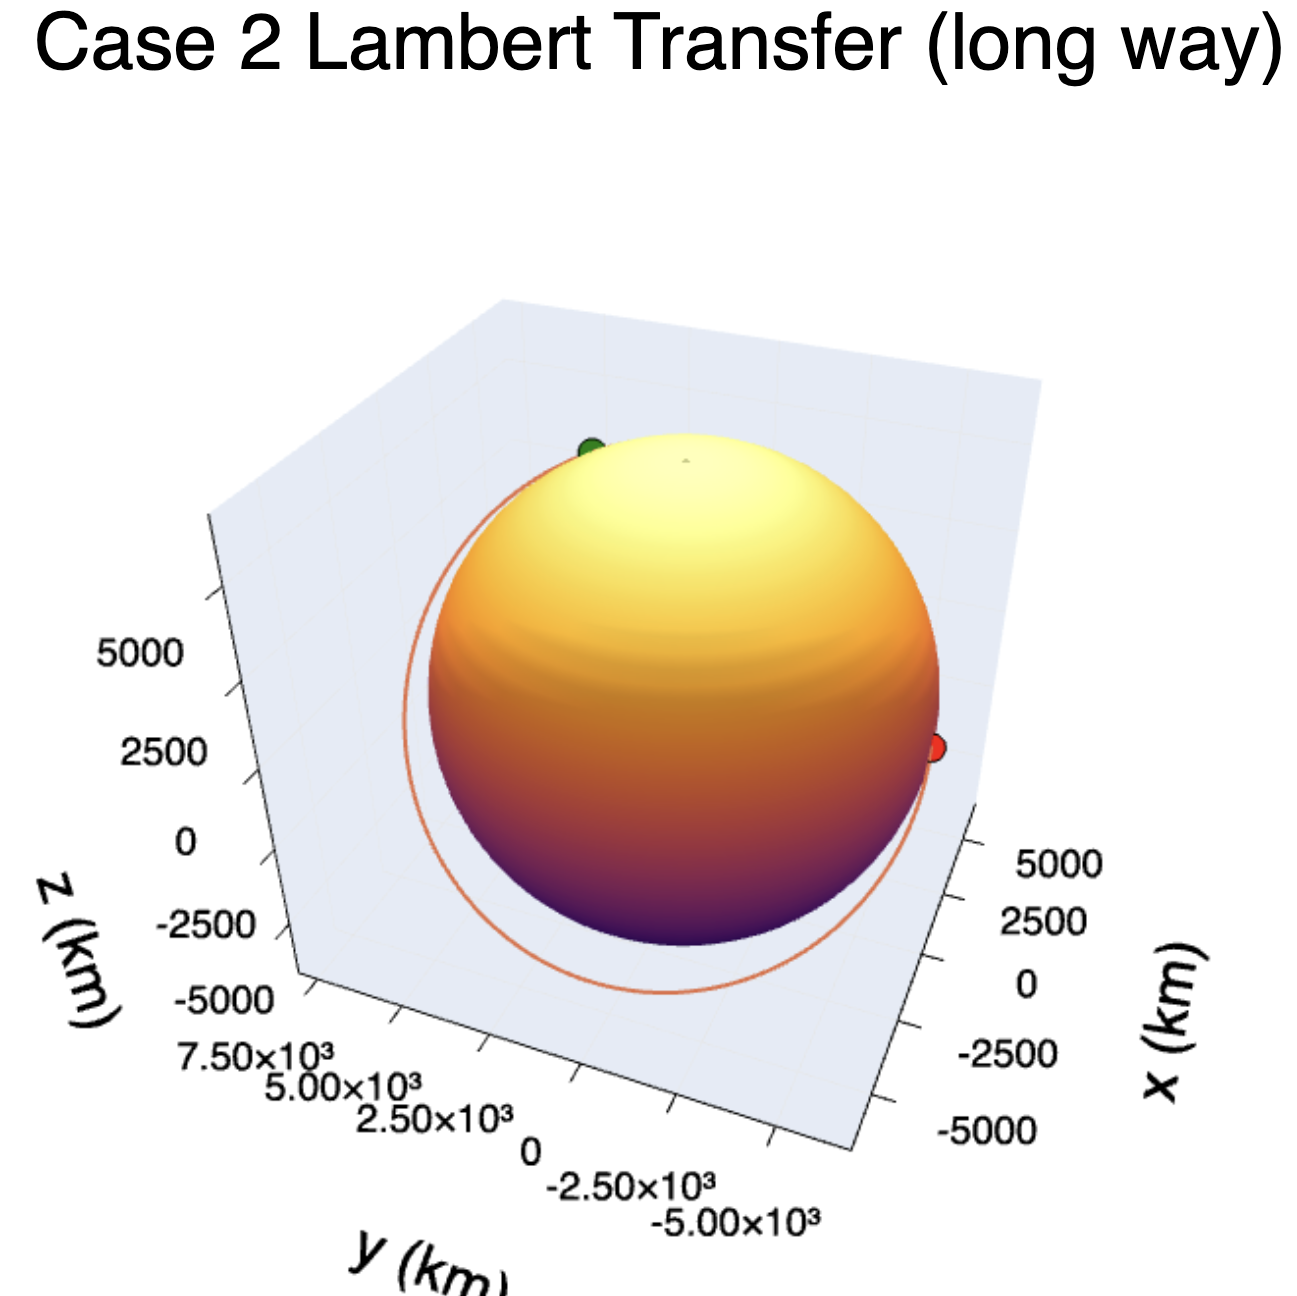
\includegraphics[width=\linewidth]{./s02c.png}


\end{document}
